\documentclass[cn,chinese,founder]{elegantbook}
\usepackage{wrapfig}
\everymath{\displaystyle}
% Useful commands:
% Add hyperlink:\href{http://example.com}{example}
%
% Adding wrapfig:
% \begin{wrapfigure}{r}{3.5cm}
%     \vspace{-1.5cm}
%     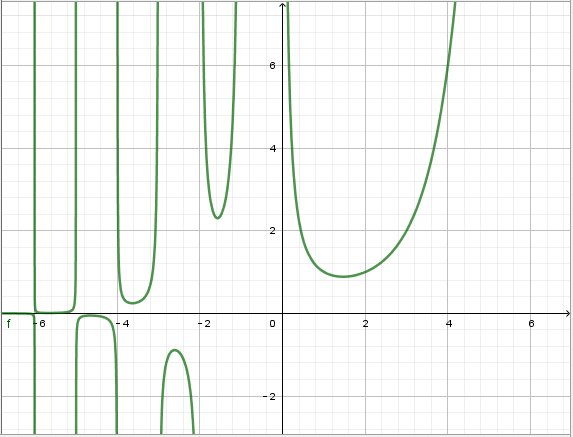
\includegraphics[width=3.5cm]{example.png}
%     \caption[示例]{示例解答图片}
% \end{wrapfigure}
% Please add it out of problem or solution envirnoment,or it behaves odd.

\begin{document}
\chapter{章节名}
 \section{节名}
  \subsection{思考题}
      \begin{example}

      \end{example}
      \begin{solution}
          解答
      \end{solution}

  \subsection{练习题}
      \begin{exercise}
          
      \end{exercise}
      \begin{solution}
          解答
      \end{solution}
\end{document}
